\documentclass[11pt]{report}
\usepackage[a4paper, margin=0.8in]{geometry}
\usepackage[french]{babel}
\usepackage[T1]{fontenc}
\usepackage{amssymb}
\usepackage{pgfplots}
\pgfplotsset{compat=1.15}
\usepackage{mathrsfs}
\usetikzlibrary{arrows}
\usepackage{amsthm}
\usepackage{amsmath}
\usepackage{stmaryrd}
\usepackage[european,straightvoltages,RPvoltages,cute inductors]{circuitikz}
\usetikzlibrary{babel}
\usepackage{listings}
\usepackage{xcolor}
\usepackage{mathtools}
\usepackage{multicol}
\usepackage{xcolor-material}
\usepackage{hyperref}
\usepackage{enumitem}
\usepackage{fancyhdr}
\usepackage{tikz}
\hypersetup{hidelinks}

\usepackage{siunitx}
\sisetup{
    locale = FR,
    separate-uncertainty,
    inter-unit-product = \cdot
}

\usepackage{pdfpages}
\usepackage{anyfontsize}
\usepackage{setspace}
\addto\captionsfrench{\renewcommand{\chaptername}{Séance}}

\allowdisplaybreaks
\setlength{\parindent}{0pt}


\newcommand{\R}{\mathbb{R}}
% Définition d'une couleur sobre pour le titre (gris très foncé)
\definecolor{darkgray}{RGB}{50, 50, 50}

\begin{document}

\begin{titlepage}
    \centering
    
    % --- En-tête ---
    \vspace*{1.5cm}
    {\LARGE \textsc{[Grenoble INP - Esisar]}}\\[1cm]
    {\Large PX222 - AUTO ELEC}\\[2cm]
    
    % --- Titre du document ---
    \textcolor{darkgray}{\rule{\linewidth}{0.8pt}} \\[0.7cm]
    {\Huge \bfseries Carnet de Bord} \\[0.4cm]
    \textcolor{darkgray}{\rule{\linewidth}{0.8pt}} \\[1.5cm]
    
    % --- Sujet ---
    {\Large \textit{Contrôle de courant dans un circuit inductif}} \\[3cm]
    
    % --- Membres du groupe (alignés à gauche) ---
 
    Antton Chevrier \quad Lucas Fernandez \quad Francis Ferguson 
    
    \vfill 
    
    \begin{flushright} \large
        \textbf{Période :} Mars à juin 2026 \\[0.4cm]
        \textit{Dernière mise à jour : \today} 
    \end{flushright}
    
\end{titlepage}

\clearpage

\tableofcontents

\clearpage

\chapter*{Introduction}
L'objectif de ce projet est de réaliser un asservissement de courant dans un circuit inductif, au travers de la bobine étudiée en PX221. Nous utilserons un microcontrôleur STM-32 pour réaliser l'asservissement numérique. 

\begin{figure}[h]
  \begin{center}
    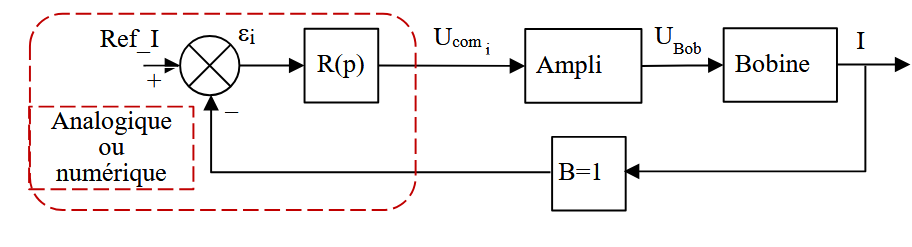
\includegraphics[width=\textwidth]{img/schema_bloc_complet.png}
    \caption{Schéma bloc du montage à réaliser}
  \end{center}
\end{figure}

\chapter{Mercredi 18 mars 2026}
\section{Modélisation des éléments du montage}
Pour commencer, nous avons modélisé les différents éléments du montage à l'aide de leurs fonctions de transfert respectives.
\subsection{Bobine}
Pour trouver la fonction de transfert de la bobine, nous pouvons la modéliser comme un circuit RL, couplé à une résistance de puissance de \qty{12}{\ohm} en série afin de pouvoir par la suite diviser la constante de temps par 2. D'après le PX221 du premier semestre, nous savons également que la résistance de la bobine est de \qty{14}{\ohm} et que son inductance est de \qty{1,2}{\henry}.

\begin{circuitikz}
  \draw (0,0) 
      to[vsource, v=$U$] (0,3)
      to [R, l=$R_{pu}$, v<=$U_{R_{pu}}$] (2,3)
      to[R, l=$R$, v<=$U_R$, i=$I$] (5,3)
      to [L, v^=$U_L$] (5,0) --(0,0) ;
\end{circuitikz}

On a alors $U=RI + R_{pu} I + ZI$ avec $Z=jL\omega$. On obtient donc $U=I(R+R_{pu}+jL\omega)$.

Sachant que la bobine prend en entrée la tension $U$ est en sortie le courant $I$, on obtient la fonction de tranfert :
\begin{align*}
  H_B(p) = \frac{I}{U} &= \frac{1}{R+R_{pu}+Lp}\\
                     &= \frac{\frac{1}{R+R_{pu}}}{1 + \frac{R+R_{pu}}{L}p} \\
                H_B(p) &= \frac{H_0}{1+\tau p} \quad \text{avec } H_0 = \frac{1}{R+R_{pu}} \text{ et } \tau = \frac{L}{R+R_{pu}}
\end{align*}

\clearpage
\subsection{Amplificateur}
\begin{figure}[h]
  \begin{center}
    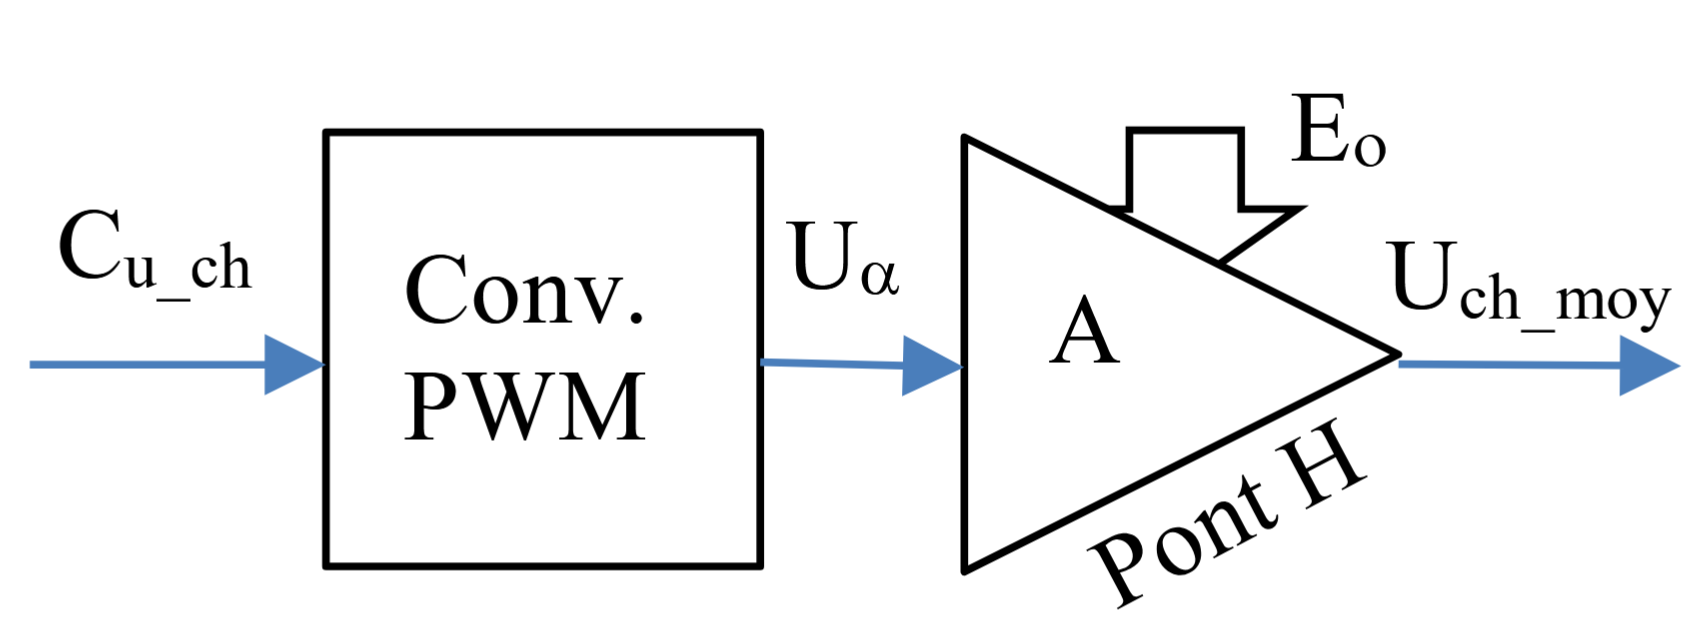
\includegraphics[width=0.3\textwidth]{img/ampli_schema_bloc.png}
    \caption{Schéma bloc fonctionnel de l'amplificateur}
  \end{center}
\end{figure}
On sait grâce au sujet que la sortie de l'amplificateur est donnée par :
\begin{equation*}
  U_{ch_{moy}} = (2 C_{u\_ch} - 1)E_0
\end{equation*}
Dans notre cas, on a $C_{u\_ch} = U_{com}$ et $C_{h_{moy}} = U_{bob}$ 

Ainsi on peut écrire la fonction de transfert de l'amplificateur : 
\begin{align*}
  H_A(p) = \frac{U_{bob}}{U_{com}} = \frac{(2 U_{com} - 1)E_0}{U_{com}} = E_0(2 - \frac{1}{U_{com}})
\end{align*}

\subsection{Calcul de la boucle ouverte}
Afin de pouvoir calculer le correcteur à mettre en place, nous allons calculer la fonction de transfert du système complet en boucle ouverte.

\begin{align*}
  H_{BO}(p) &= R(p) \cdot K_A \cdot H_B(p) \cdot B \quad\quad \text{avec $K_A$ le gain de l'amplificateur}\\ 
            &= k(2E_0) \cdot \frac{\frac{1}{R + R_{pu}}}{1+\tau p} \\
            &= \frac{\frac{2kE_0}{R+R_{pu}}}{1+\tau p}
\end{align*}



\section{Pour la prochaine séance}
Nous devrons avoir terminé les calculs des fonctions de transfert en boucle ouvertes et fermée, ainsi que le calcul du correcteur proportionnel.

\end{document}